\chapter{Asking Orlando Millionaires How They Got Rich}

This lecture is built as a chain of interviews rather than as a single uninterrupted exposition, but it still unfolds with a clear analytic order. We begin with scale claims and learning costs, move to a decision rule about value and price, widen into business design and wealth structure, descend into the problem of escaping the poverty cycle, and close with credit as a lever of operational expansion. The mathematics here is modest and practical rather than formal: it is the arithmetic of leverage, allocation, compounding, and foregone upside.

\section{Cold Open and Conference Frame}

The opening montage gives us the lecture in compressed form. A mentor is said to have cost \$55{,}000 and helped scale a business above \$5 million a year. We hear single-year revenue claims in the eight-figure range. We also hear, almost in passing, the question that will organize much of what follows: how do wealthy people think about money differently?

Only after this teaser does the host reset the scene. We are in Orlando, at Funnel Hacking Live, and the method of the lecture is made explicit: we will hear a sequence of entrepreneurs describe how they made money, what choices created wealth in their industries, and what a viewer can do to begin moving in the same direction. This reset matters. The montage creates appetite; the conference frame turns that appetite into inquiry.

The lecture then proceeds by sampling. We are not given one master doctrine up front. We are given a set of local mechanisms, each attached to a speaker, and the chapter should preserve that serial motion rather than flattening it into a single abstract essay.

\section{Scale, Learning, and the Right to Generalize}

The first interviewee, who says he runs a marketing agency, is introduced through scale. The host asks what the most money is that he has made in a single year. The answer is about \$13 million. We are also told that he has been a business owner for fifteen years, and that roughly \$500{,}000 was spent learning to sell, learning to market, and entering masterminds. The speaker then states the resulting number plainly: that spend turned into \$33 million.

This is one of the lecture's first real calculations. The speaker is not saying that all education pays off, nor that the number is profit. He is saying that he treated learning as productive capital rather than as luxury consumption.

\begin{equation}
C_{\text{learn}}=\$500{,}000,
\qquad
R_{\text{learn}}=\$33{,}000{,}000,
\qquad
m_{\text{learn}}=\frac{R_{\text{learn}}}{C_{\text{learn}}}=66.
\end{equation}

The host continues to collect large numerical claims across the episode, and it is useful to keep them visible as part of the lecture's rhythm. They function as credibility markers before each speaker is allowed to generalize.

\begin{table}
\centering
\begin{tabular}{ll}
Claimed magnitude & Context \\
\hline
about \$13 million & first interviewee, single year \\
about \$18 million & Marcus, single year \\
about \$25 million & all companies combined / stage milestone \\
about \$10--11 million & projected best year for final speaker \\
about \$20--25 million & Eddie's business this year \\
\end{tabular}
\end{table}

The lecture is careful, in its own way, about sequence. First we are shown that these speakers operate at scale. Only then do we ask what rules of thought produced that scale.

\section{Value Before Price}

The host now zooms out. He asks what separates the middle class from the wealthy in the way people look at money. The answer is not first given as theory. It is given as a staged problem with a bag.

\subsection{Question \& Answer}

\paragraph{Question.} What is the most important difference in how poor and wealthy people evaluate money?

\paragraph{Answer.} The poor answer the wrong question first. They hear a price and react to the price. The wealthy ask what is inside.

The bag analogy is simple enough to write down. A bag is offered for \$1{,}000. The listener says he would probably pass. The speaker then inserts the hidden variable: suppose the bag contains \$100{,}000 in cash. The economic mistake is now obvious.

\begin{equation}
P_{\text{bag}}=\$1{,}000,
\qquad
V_{\text{inside}}=\$100{,}000,
\qquad
U_{\text{bag}}=V_{\text{inside}}-P_{\text{bag}}=\$99{,}000.
\end{equation}

This is the lecture's cleanest decision rule. Before we decide whether something is expensive, we ask what it is worth. The speaker's phrasing is memorable because it reverses the usual order of attention: rich people worry about what they get, not what it costs.

That rule also clarifies the function of the opening montage. The very first numbers we heard were meant to train the ear away from sticker shock and toward leverage. A \$55{,}000 mentorship sounds expensive until it is compared with the scale it allegedly helped produce.

\section{Sales, Brand, and Coherence}

Having used the bag to discuss money perception, the host asks about sales. Here the lecture makes a sharp pivot. Instead of offering a tactic for closing deals, the speaker recasts the question as one of brand design. He asks what the most enduring personal brands of all time are, answers with superheroes, and then explains why: superheroes stand clearly for something and clearly against something.

The movement is important. We go from transaction to identity. A strong brand, in the speaker's language, is not a surface label; it is a stable partition of conduct. One may adapt an existing archetype, as he says he adapted Iron Man into ``Iron Dan,'' but the power comes from consistency.

If we introduce notation merely as a shorthand, not as a claim about what the speaker literally wrote, we may let \(\mathcal{F}\) denote what the brand stands for and \(\mathcal{G}\) denote what it stands against. Then a public statement or action \(a\) is coherent only if it aligns with that pair.

\begin{equation}
\chi_{\text{brand}}(a)=1
\iff
a \text{ aligns with }(\mathcal{F},\mathcal{G}).
\end{equation}

This editorial notation captures the lecture's core point: ``everything you say, everything you do'' must fall into alignment with the declared structure of the brand. The transcript becomes garbled when the speaker turns to harsh examples about ignorance and business seriousness, so we should not over-clean that passage. But the mechanism is clear enough. Brand is repeated alignment.

The host's response is also part of the lecture's logic. He pauses, praises the interview, and says in effect that the analogies revealed how poor people think: they do not ask the right questions. That recap is not ornamental. It is the lecture's first explicit consolidation point.

\section{Recession-Proof Structure and the Architecture of Wealth}

The next interview begins with another visible prompt. The host notices Marcus's shirt and asks for a blueprint to build a recession-proof business. The answer is again architectural rather than psychological. A business should make money three or four ways; better yet, it should have at least four verticals.

\begin{equation}
n_{\text{verticals}}\ge 4.
\end{equation}

The lecture gives a concrete decomposition: the core product or service, a digital product, an in-person event, and a high-ticket mentorship or program. The arithmetic is small enough to see the point clearly. If the high-ticket program costs \$50{,}000 and only four people take it in a year, that one vertical alone contributes \$200{,}000.

\begin{equation}
P_{\text{high-ticket}}=\$50{,}000,
\qquad
N=4,
\qquad
R_{\text{high-ticket}}=P_{\text{high-ticket}}N=\$200{,}000.
\end{equation}

\begin{figure}
\centering
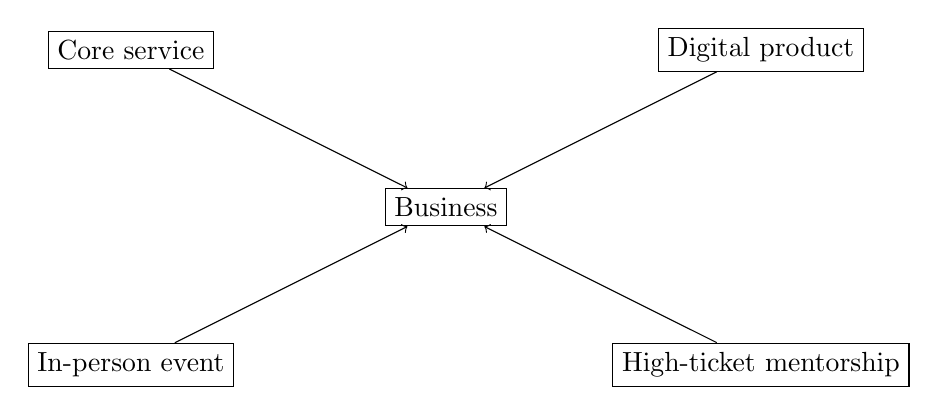
\begin{tikzpicture}
\node[draw, rectangle] (biz) at (0,0) {Business};
\node[draw, rectangle] (core) at (-4,2) {Core service};
\node[draw, rectangle] (digital) at (4,2) {Digital product};
\node[draw, rectangle] (event) at (-4,-2) {In-person event};
\node[draw, rectangle] (mentor) at (4,-2) {High-ticket mentorship};

\draw[->] (core) -- (biz);
\draw[->] (digital) -- (biz);
\draw[->] (event) -- (biz);
\draw[->] (mentor) -- (biz);
\end{tikzpicture}
\end{figure}

The lecture then turns, very naturally, from business durability to personal wealth. Marcus says that wealth is not determined by dollar amount but by structure. This is a crucial shift. Up to now the numbers have mostly been top-line revenue claims. Here we move into allocation.

If annual earned income is \(Y\), with savings rate \(s\), then the annual savings flow is \(S=sY\). The lecture uses the example \(Y=\$100{,}000\) and \(s\in[0.20,0.25]\), so that

\begin{equation}
S=sY\in[\$20{,}000,\$25{,}000].
\end{equation}

But the speaker insists that savings alone is not the whole story. What matters is the way money is divided among positions that grow: real-estate equity, investment portfolio, and retained or reinvestable cash. A cautious summary of the mechanism is

\begin{equation}
\Delta W \approx S+\Delta E_{\mathrm{RE}}+\Delta A_{\mathrm{inv}}+CF_{\mathrm{ret}}.
\end{equation}

This is not a board formula from the lecture; it is a bookkeeping identity extracted from the spoken list. Still, it lets us say exactly what the lecture is trying to say. Wealth is not merely high income. Wealth is a system in which income is translated into appreciating or compounding components.

The host again marks the transition. He praises Marcus, cites the \$18 million figure, and extracts the slogan that a business must survive beyond whatever the outside world and the economy happen to be doing. That breath in the lecture prepares the next pivot.

\section{Offense, Deployment, and the Poverty Trap}

The Eddie interview turns from structure to posture. The host asks, once again, about the difference between the middle class and those who build generational wealth. Eddie answers with a pair of animal and military images. Poor people, he says, behave like squirrels storing acorns. Rich people treat dollars like soldiers and send them out to bring back more dollars.

We should not force this into false precision, but the distinction is sharp enough. Defense means preserving the present stock. Offense means deploying the stock in ways that change the future state. The lecture emphasizes this not as a balance-sheet theorem but as a behavioral asymmetry: some people hoard and hide, while others invest, build, and widen the field of action.

The host then narrows the problem. Instead of asking about wealth in general, he asks what a person stuck in a cycle of poverty should do first. This is the lecture's strongest local tension, and it deserves to remain explicit.

\subsection{Question \& Answer}

\paragraph{Question.} If one is trapped in the cycle of poverty, what is the first practical move?

\paragraph{Answer.} The answer is given as a time-structured trade. The speaker says that when he was \(21\), he left a sales job paying about \$150{,}000 a year for a job paying about \$30{,}000 a year, because the lower-paying path offered more learning.

The immediate numerical consequence is negative:

\begin{equation}
\Delta Y_0
=
Y_{\text{learning job}}-Y_{\text{sales job}}
\approx
30{,}000-150{,}000
=
-\$120{,}000.
\end{equation}

If we stop there, the choice looks irrational. But the lecture insists that the real state variable is not current wage income; it is human capital. Let \(H_t\) denote accumulated skill, judgment, and commercially usable knowledge at time \(t\). Then the mechanism is

\begin{align}
H_{t+1} &= H_t+\Delta H_t, \\
Y_t &= f(H_t), \qquad f'(H_t)>0.
\end{align}

The point is not that every low-paying job is secretly better. The point is that, early in life, a path with larger \(\Delta H_t\) may dominate a path with larger current \(Y_t\). The speaker's claim is that the later annual payoff can become so large that it dwarfs what would have been earned by chasing wages too early.

The sequence is pedagogically precise:

\begin{enumerate}
\item accept a short-run income sacrifice;
\item direct time and money into knowledge, information, and saleable skills;
\item allow those skills to compound rather than stagnate;
\item collect the later earnings when the market now pays for accumulated competence.
\end{enumerate}

This is why the lecture returns again and again to paid learning, masterminds, courses, and mentors. Knowledge is treated not as ornament but as a capital input with delayed yield.

The final exhortation in this segment is rhetorically intense, but the analytic point is simple: if one is not where one wants to be, then the scarce resources of time and attention must be redirected into learning and execution rather than passive consumption.

\section{Credit, Mentorship, and Financial Leverage}

The final interview narrows from worldview to machinery. The speaker explains that he teaches people to start, grow, or scale a business by leveraging credit, and he claims to have built software that helps with this process. The technical description of the software is too garbled in the transcript to formalize further, so the chapter should remain cautious there.

What is clear is the lecture's sequence. First comes a critique of the standard educational path: if one learns from people earning \$40{,}000 to \$60{,}000 a year, one may reproduce only that range of outcomes. Then comes the return to mentorship, which now completes the circle opened in the teaser.

\begin{equation}
C_{\text{mentor}}=\$55{,}000,
\qquad
R_{\text{post-mentor}}\gtrsim \$5{,}000{,}000\text{/yr},
\qquad
m_{\text{mentor}}
=
\frac{R_{\text{post-mentor}}}{C_{\text{mentor}}}
\approx 90.9.
\end{equation}

We should again label this carefully. It is a gross revenue multiple claimed by the speaker, not a verified net return. The same caution applies to the later line about the business being headed toward eight figures. One transcript line is badly garbled as ``\$10{,}000, \$11{,}000 million,'' but in context it is safest to read this as a projection of about \$10--11 million.

The lecture then gives a more operational chain. A tradeline, or authorized-user line added to the credit profile, is said to affect four of five credit metrics positively. That improvement is then linked to a score movement from about \(600\) to \(700\), and that movement is linked to access to \$50{,}000 to \$100{,}000 in credit.

\begin{equation}
T
\longrightarrow
\frac{4}{5}\text{ metrics improved}
\longrightarrow
C_{\text{score}}:600\to700
\longrightarrow
L_{\text{access}}\in[\$50{,}000,\$100{,}000].
\end{equation}

We should resist the temptation to turn this into a comprehensive theory of credit scoring. The lecture does not enumerate the five metrics, and it does not present a formal scoring model. What it does present is a leverage pathway. A stronger credit profile expands available financial room; expanded financial room can be used to start, grow, or scale a business.

Seen from a higher vantage, this final section does not introduce a new philosophy. It gives a final instance of the same philosophy. Learning is leverage. Multiplying revenue streams is leverage. Deploying money offensively is leverage. Credit improvement is leverage. The lecture's unity lies there.

\section{Summary}

The lecture proceeds step by step, and the order should be respected. First we are given scale, so that the speakers can be heard as operators rather than as theorists. Then we are given the simplest rule of all: ask about value before reacting to price. From there the lecture moves outward into sales, brand coherence, business architecture, wealth allocation, offensive deployment of capital, human-capital compounding, and finally credit as an instrument of expansion.

None of this is formal finance, and none of it should be dressed up as a theorem-proving exercise. But the mathematics is real. It is the mathematics of ratios, opportunity cost, savings rates, component growth, state updates, and leverage chains. The chapter's governing verb is therefore not merely to earn, nor merely to save, but to transform: transform spending into skill, skill into revenue, revenue into structure, structure into resilience, and credit into enlarged possibility.